\documentclass[12pt, answers]{exam}
\usepackage{tikz}
\usepackage{amsmath}
\usepackage{amsfonts}
\usepackage{amssymb}
\usepackage{graphicx}
\usepackage{multirow}
\usepackage{enumitem}
\usepackage{subfiles}
\usepackage{xepersian}

\settextfont[
    Path = ../fonts/,
    Scale = 1.0,
    BoldFont = *Bd,
    ItalicFont = *It,
    BoldItalicFont = *BdIt,
    Extension = .ttf
]{XB Yas}

\renewcommand{\solutiontitle}{\noindent\textbf{\color{blue}پاسخ:}\par}
\newcommand{\class}{اصول سیستم‌های عامل}
\newcommand{\term}{نیم‌سال اول ۰۴-۰۵}
\newcommand{\college}{دانشکده ریاضی و آمار}
\newcommand{\prof}{استاد: دکتر رفیعی}
\newcommand{\group}{نام دانشجو}

\begin{document}
%%%%%%%%%%%%%% HDR START 
\pagestyle{head}
\firstpageheader{}{}{}
\runningheader{صفحه \thepage\ از \numpages}{}{\class}
\runningheadrule
\begin{tabular}{p{.7\textwidth} l}
    \multicolumn{2}{c}{\textbf{به نام خدا}}                                            \\
                    & \multirow{2}{*}{
\includegraphics[scale=0.2]{../UILOGO.png}} \\
    \textbf{\class} &                                                                  \\
    \textbf{\term}  &                                                                  \\
    \textbf{\prof}  &                                                                  \\
    \textbf{\group} &                                                                  \\
                    & \textbf{\college}                                                \\
    % & \textbf{\todaydate} \\
    % & \textbf{\deadline} \\ \\
\end{tabular}\\
\rule[1ex]{\textwidth}{.1pt}

\begin{center}
    \textbf{\lr{Problem Set 1}}
\end{center}
%%%%%%%%%%%%%% HDR END 


\begin{questions}
    \pointpoints{نمره}{نمره}

    %%%%%%%%%%%%%% 1 START 
    \question به سوالات زیر پاسخ کامل دهید:
\begin{parts}
    \part[5]  تفاوت سیستم‌های خوشه‌ای و سیستم‌های چند پردازنده‌ای چیست؟ دو ماشین متعلق به یک خوشه چه همکاری‌ای باید داشته باشند تا سرویس خوبی فراهم شود؟
    \part[5]  هدف وقفه چیست؟ تفاوت‌های بین وقفه و تله چیست؟ آیا تله می‌تواند به دلخواه توسط برنامه‌نویس تولید شود؟ اگر بلی، برای چه هدفی؟
    \part[5]  معماری NUMA چیست و چرا زمان دسترسی پردازنده‌ها به حافظه در این معماری یکسان نیست؟
    \part[10]  در چه حالتی استفاده از چندبرنامگی به جای چند وظیفگی راندمان سیستم کامپیوتری را افزایش می‌دهد؟
    چنین سیستمی برای چه کارهایی مناسب‌تر است؟
\end{parts}


    \begin{solution}
        جواب خود را اینجا بنویسید.
    \end{solution}
    %%%%%%%%%%%%%% 1 END 

    \pagebreak

    %%%%%%%%%%%%%% 2 START
    \question[20]  تصور کنید شما طراح یک سیستم‌عامل جدید هستید و به دلایل عملکردی تصمیم گرفته‌اید اجرای دو حالته
    (\lr{User Mode} و \lr{Kernel Mode})
    را حذف کنید. در این سیستم همه برنامه‌ها مستقیماً به سخت‌افزار و حافظه کامل دسترسی دارند.
    \begin{enumerate}
        \item تحلیل کنید چه مشکلات امنیتی، پایداری و همزمانی ممکن است ایجاد شود.
        \item توضیح دهید یک برنامه مخرب چگونه می‌تواند از این ضعف برای دسترسی به حافظه برنامه‌های دیگر، خراب کردن فایل‌ها یا مختل کردن سیستم سوءاستفاده کند.
        \item اگر بخواهید بدون برگرداندن حالت کرنل، سطحی از امنیت و کنترل منابع را حفظ کنید، چه روش‌های جایگزینی پیشنهاد می‌کنید؟
        \item توضیح دهید اجرای دو حالته چگونه این مشکلات را به شکل ساده‌تر و مؤثرتری حل می‌کند.
    \end{enumerate}

    \begin{solution}
        جواب خود را اینجا بنویسید.
    \end{solution}
    %%%%%%%%%%%%%% 2 END

    \pagebreak

    %%%%%%%%%%%%%% 3 START
    
\question آقا
طرفای صفحه ۸ اسلاید ۴ یه دیاگرامی بود که خیلی شیک اسکیپ کردید. چی میگفت
حالا؟ داشت نشون می‌داد که اگر وسط کار
CPU
عزیز یه وقفه ایجاد بشه، روند انجام کارها به چه صورت پیش می‌رِد!
چون حوصله باز کردن اسلاید‌ها رو ندارید عکسشو میذاریم اینجا:
\begin{center}
    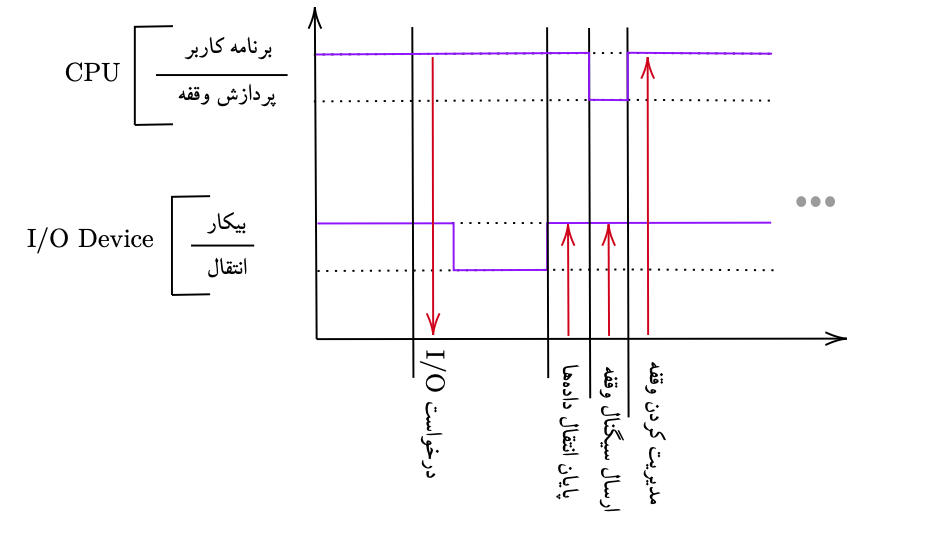
\includegraphics[scale=0.9]{images/diagram.png}
\end{center}

اول خوب تحلیلش کنید و بعد سناریوی زیر رو بخونید:
\begin{enumerate}
    \item یک فرایند کاربر که روی CPU در حال اجراست، یک درخواست ورودی/خروجی (I/O) به دیسک ارسال می‌کند. به جای اینکه CPU هر انتقال داده را با وقفه‌ها مدیریت کند، از
          \lr{DMA (Direct Memory Access)}
          استفاده می‌کند.
    \item وقتی درخواست I/O داده می‌شود، CPU کنترلر DMA را برنامه‌ریزی کرده و سپس اجرای فرایند کاربر را ادامه می‌دهد.
    \item کنترلر DMA انتقال داده‌ها بین حافظه و دستگاه ورودی/خروجی را مستقیماً برعهده می‌گیرد، در حالی که CPU آزاد است تا دستورهای کاربر را اجرا کند.
    \item وقتی انتقال کامل شد، کنترلر DMA یک وقفه به CPU می‌فرستد. CPU به‌طور کوتاه وقفه را رسیدگی کرده و سپس اجرای فرایند کاربر را از سر می‌گیرد.
\end{enumerate}

\begin{parts}
    \pagebreak
    \part[15] حالا با توجه به سناریوی بالا، دیاگرام پایین رو کامل کنید.

    % \vspace{1cm}
    \begin{center}
        \scalebox{0.8}{ 
\tikzset{every picture/.style={line width=0.75pt}} %set default line width to 0.75pt        

\begin{tikzpicture}[x=0.75pt,y=0.75pt,yscale=-1,xscale=1]
%uncomment if require: \path (0,455); %set diagram left start at 0, and has height of 455

%Straight Lines [id:da23411427234450732] 
\draw    (130,20.96) -- (130,130.96) ;
%Straight Lines [id:da2889349755532342] 
\draw    (197,50.96) -- (130,50.96) ;
%Straight Lines [id:da21977095406729874] 
\draw    (196,90.96) -- (149,90.96) -- (130,90.96) ;
%Straight Lines [id:da31310232070946165] 
\draw    (130,159.02) -- (130,220.46) ;
%Straight Lines [id:da07562191549324238] 
\draw    (197,191) -- (130,191) ;
%Straight Lines [id:da976549806276633] 
\draw    (130,262) -- (130,325.96) ;
%Straight Lines [id:da8117752926288655] 
\draw    (197,292) -- (130,292) ;
%Straight Lines [id:da8258334393782207] 
\draw    (250,330.46) -- (250,6.46) ;
\draw [shift={(250,4.46)}, rotate = 90] [color={rgb, 255:red, 0; green, 0; blue, 0 }  ][line width=0.75]    (10.93,-3.29) .. controls (6.95,-1.4) and (3.31,-0.3) .. (0,0) .. controls (3.31,0.3) and (6.95,1.4) .. (10.93,3.29)   ;
%Straight Lines [id:da8335872942840874] 
\draw    (250,330.46) -- (648,329.47) ;
\draw [shift={(650,329.46)}, rotate = 179.86] [color={rgb, 255:red, 0; green, 0; blue, 0 }  ][line width=0.75]    (10.93,-3.29) .. controls (6.95,-1.4) and (3.31,-0.3) .. (0,0) .. controls (3.31,0.3) and (6.95,1.4) .. (10.93,3.29)   ;
%Straight Lines [id:da12472960327209215] 
\draw  [dash pattern={on 0.84pt off 2.51pt}]  (260,269) -- (633,269) ;
%Straight Lines [id:da3649012449780963] 
\draw  [dash pattern={on 0.84pt off 2.51pt}]  (259,309) -- (632,309) ;
%Straight Lines [id:da15102065785650298] 
\draw  [dash pattern={on 0.84pt off 2.51pt}]  (261,169) -- (634,169) ;
%Straight Lines [id:da5497552300455996] 
\draw  [dash pattern={on 0.84pt off 2.51pt}]  (260,209) -- (633,209) ;
%Straight Lines [id:da13915645381980746] 
\draw  [dash pattern={on 0.84pt off 2.51pt}]  (259,69) -- (632,69) ;
%Straight Lines [id:da7002272418046886] 
\draw  [dash pattern={on 0.84pt off 2.51pt}]  (258,109) -- (631,109) ;
%Straight Lines [id:da5752524111385351] 
\draw  [dash pattern={on 0.84pt off 2.51pt}]  (259,29) -- (632,29) ;
%Straight Lines [id:da473783091142272] 
\draw    (309,30) -- (309,361.46) ;
%Straight Lines [id:da6306032256053173] 
\draw    (445.5,29) -- (445.5,360.46) ;
%Straight Lines [id:da04262266935154879] 
\draw    (475.5,29) -- (475.5,360.46) ;
%Straight Lines [id:da33011764463887383] 
\draw    (505.5,29) -- (505.5,360.46) ;

% Text Node
\draw (85,64) node [anchor=north west][inner sep=0.75pt]   [align=left] {\begin{minipage}[lt]{24.26pt}\setlength\topsep{0pt}
\begin{flushright}
CPU
\end{flushright}

\end{minipage}};
% Text Node
\draw (147,21.96) node [anchor=north west][inner sep=0.75pt]   [align=left] {\begin{minipage}[lt]{44.53pt}\setlength\topsep{0pt}
\begin{flushright}
\begin{RTL}
    برنامه کاربر
\end{RTL}

\end{flushright}

\end{minipage}};
% Text Node
\draw (147,101.96) node [anchor=north west][inner sep=0.75pt]   [align=left] {\begin{minipage}[lt]{52pt}\setlength\topsep{0pt}
\begin{flushright}
\rl{پردازش وقفه}
\end{flushright}

\end{minipage}};
% Text Node
\draw (147,61.96) node [anchor=north west][inner sep=0.75pt]   [align=left] {\begin{minipage}[lt]{73pt}\setlength\topsep{0pt}
\begin{flushright}
    \begin{RTL}
        برنامه‌ریزی DMA
    \end{RTL}
\end{flushright}

\end{minipage}};
% Text Node
\draw (85,185.04) node [anchor=north west][inner sep=0.75pt]   [align=left] {\begin{minipage}[lt]{25.39pt}\setlength\topsep{0pt}
\begin{flushright}
DMA
\end{flushright}

\end{minipage}};
% Text Node
\draw (147,166) node [anchor=north west][inner sep=0.75pt]   [align=left] {\begin{minipage}[lt]{20.28pt}\setlength\topsep{0pt}
\begin{flushright}
بیکار
\end{flushright}

\end{minipage}};
% Text Node
\draw (147,199) node [anchor=north west][inner sep=0.75pt]   [align=left] {\begin{minipage}[lt]{20pt}\setlength\topsep{0pt}
\begin{flushright}
انتقال
\end{flushright}

\end{minipage}};
% Text Node
\draw (46,285.04) node [anchor=north west][inner sep=0.75pt]   [align=left] {\begin{minipage}[lt]{55.34pt}\setlength\topsep{0pt}
\begin{flushright}
    \begin{LTR}
        I/O Device
    \end{LTR}
\end{flushright}

\end{minipage}};
% Text Node
\draw (147,263) node [anchor=north west][inner sep=0.75pt]   [align=left] {\begin{minipage}[lt]{20.28pt}\setlength\topsep{0pt}
\begin{flushright}
بیکار
\end{flushright}

\end{minipage}};
% Text Node
\draw (147,303) node [anchor=north west][inner sep=0.75pt]   [align=left] {\begin{minipage}[lt]{20pt}\setlength\topsep{0pt}
\begin{flushright}
انتقال
\end{flushright}

\end{minipage}};
% Text Node
\draw (330.79,340) node [anchor=north west][inner sep=0.75pt]  [rotate=-90] [align=left] {\begin{minipage}[lt]{60pt}\setlength\topsep{0pt}
\begin{flushright}
    \begin{RTL}
        درخواست I/O
    \end{RTL}
\end{flushright}

\end{minipage}};
% Text Node
\draw (467,344.95) node [anchor=north west][inner sep=0.75pt]  [rotate=-90] [align=left] {\begin{minipage}[lt]{45pt}\setlength\topsep{0pt}
\begin{flushright}
    \begin{RTL}
        پایان انتقال
    \end{RTL}
\end{flushright}

\end{minipage}};
% Text Node
\draw (496,336) node [anchor=north west][inner sep=0.75pt]  [rotate=-90] [align=left] {\begin{minipage}[lt]{85pt}\setlength\topsep{0pt}
\begin{flushright}
    \begin{RTL}
        ارسال سیگنال وقفه
    \end{RTL}
\end{flushright}

\end{minipage}};
% Text Node
\draw (525,345) node [anchor=north west][inner sep=0.75pt]  [rotate=-90] [align=left] {\begin{minipage}[lt]{75pt}\setlength\topsep{0pt}
\begin{flushright}
    \begin{RTL}
        پایان پردازش وقفه
    \end{RTL}
\end{flushright}

\end{minipage}};


\end{tikzpicture}
}
    \end{center}

    \part[5] فرق حالتی که از DMA استفاده می‌کنیم با حالتی که ازش استفاده نمی‌کنیم چیه؟
    آیا میزان زمانی که
    CPU
    درگیر میشه تغییری می‌کنه؟ توضیح بدین.

\end{parts}

    \begin{solution}
        جواب خود را اینجا بنویسید.
    \end{solution}
    %%%%%%%%%%%%%% 3 END

    \pagebreak

    %%%%%%%%%%%%%%% 4 START
    \question کیومرث چند وقته که حس می‌کنه ویندوزش
دیر بالا میاد. برای رفع این مشکل تصمیم گرفته تا یکی از عجیب‌ترین راه‌حل‌های ممکن
رو امتحان کنه
(منظورمون نصب
Arch
نیست):

اون می‌خواد حافظه‌ای که برنامه بوت‌استرپ روی اون قرار گرفته رو با یک حافظه‌ی سریعتر
جایگزین کنه. با فرض اینکه واقعا انجام این کار سرعت رو بالا ببره به سوالات زیر جواب بدین.
\begin{parts}
    \part[10] کیومرث چه نوع حافظه‌ای رو میتونه برای این کار استفاده کنه؟ (توی این قسمت از سوال فقط سرعت مهمه)
    \part[10] به نظر شما کیومرث چه چیزی رو داره از قلم میندازه؟ آیا حافظه‌ای که در قسمت الف
    معرفی کردین واقعا میتونه جایگزین مناسبی برای
    \textbf{حافظه فقط‌خواندنی}
    باشه؟ چرا؟
    (دو دلیل بیارین)
\end{parts}

    \begin{solution}
        جواب خود را اینجا بنویسید.
    \end{solution}
    %%%%%%%%%%%%%%% 4 END

    \pagebreak

    %%%%%%%%%%%%%%% 5 START
    \question[15] با درنظر گرفتن این موضوع که تعریف دقیقی از ماهیت سیستم‌عامل وجود ندارد، اما اغلب آنها ویژگی‌های زیر را دارند:
\begin{parts}
    \part زمان و سطح دسترسی هریک از نرم‌افزارها رو به سخت‌افزار مدیریت می‌کند.
    \part برنامه‌ای است که همیشه درحال اجرا است.
    \part مانند پلی بین سخت‌افزار و نرم‌افزار عمل می‌کند.
\end{parts}
دلیل وجود هریک از آنها را توجیه کنید.
آیا میتوان سیستم‌عاملی ساخت که حداقل یکی از این ویژگی‌ها را نداشته باشد؟ اگر جواب مثبت است، چنین سیستمی با چه چالش‌هایی مواجه است؟


    \begin{solution}
        جواب خود را اینجا بنویسید.
    \end{solution}
    %%%%%%%%%%%%%%% 5 END
\end{questions}
\end{document}